\section{Results}
\begin{doublespacing}
In this study, heat conduction simulations were used to study the impact of overall heat transfer coefficient in the presence of Xenon bubble in the intragranular region. Grain boundary resistance and the influence of intergranular fission is not included in this calculation. This simulation is design to see the impact on heat transfer due to the formation of Gas Bubble Superlattice. Bubble superlattice formation inside U-Mo fuel stabilizes the fuel swelling behavior but heavily impacts the heat transfer capability~\cite{burkes2015thermal}. This might be due to Xenon's very low thermal conductivity. Thermal properties of Xenon was also considered in this work. Xenon's thermal conductivity is function of both temperature and pressure~\cite{rabinovich1987thermophysical}. Since the size the of the bubble changes with the burnup and fission density, thermal conductivity of the bubble also changes~\cite{miller2012advantages}. Pressure inside the bubble is highly depend on the curvature of the bubble.

\begin{figure}[H]
\centering
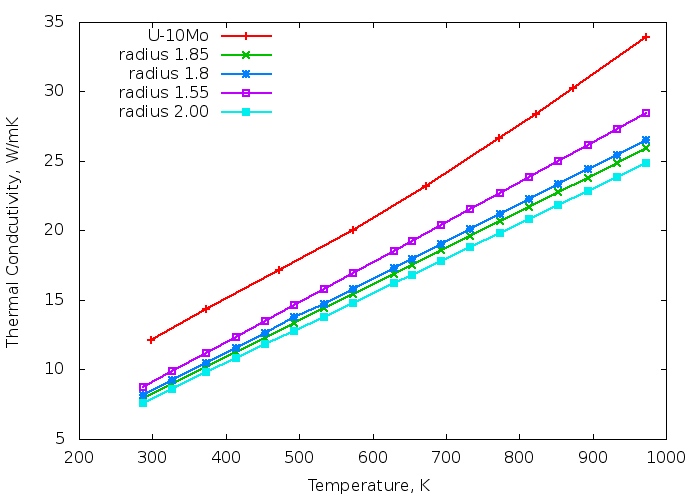
\includegraphics[scale=0.5]{result_Xe_U-10Mo.png}
\caption{Comparison between the thermal conductivity of U-10Mo and the inclusion of Xe bubble of different sizes}
\label{fig_result}
\end{figure}

FEM calculations were performed on \ref{fcc_mesh} in order to calculate the thermal flux and the thermal conductivity in 2D. 

\end{doublespacing}
